%%%%%%%%%%%%%%%%%%%%%%%%%%%%%%%%%%%%%%%%%%%%%%%%%%%%%%%
% Please note that whilst this template provides a
% preview of the typeset manuscript for submission, it
% will not necessarily be the final publication layout.
% This sample article template text was last updated 9 February 2018.
%
\documentclass[lineno]{asm-article}

\usepackage{blindtext}

\usepackage{chemformula}
\usepackage{siunitx}

\title{This Is the Sample Article Template for \textit{mSystems}\textsuperscript{\textregistered}, an American Society for Microbiology (ASM) Journal}

%%% Use \authfn{<n>} to annotate authors for present addresses.
%%% \authfn{1} is reserved for corresponding author.
\author{%
  First Author,\afn{a}
  Second Author,\afn{a,\authfn{2}}
  Third Author,\afn{b}
  Fourth Final Author,\afn{a,b,\authfn{1}}
}

\affil{%
  University Name, Faculty Group, Department, City, Country\afn{a};
  Company Name, City, Country\afn{b}
}

% Running author should not exceed 54 characters and spaces
\runningauthor{FirstAuthor et al.}
\runningtitle{Running Title}

\corraddress{Fourth Author, fourth@author.edu}

%% Use the corresponding \authfn{<n>} to state present address of marked author.
\presentaddress{\authfn{2} Present Address: Second Author, Full Affiliation.
\par
Co-first Authors.  If more than one co-first author is designated, authors are required to state how the order of names was decided as an additional footnote on the title page. See the example in the author line above.
}

%% State co-first authorship information here.
\equalcontrib{Third Author and Fourth Author contributed equally. First Author and Second Author contributed equally to this work. Author order was determined XXXXXX.}

%% LEAVE THIS FIELD EMPTY; it will only be assigned
%% during the peer review stage.
% \paperfield{}

%% Choose the appropriate paper type
\papertype{Research Article}
%\papertype{Resource Report}
%\papertype{Methods and Protocols}

\hyphenation{poly-leu-cine Ber-gey}

\begin{document}

\maketitle

%%% %TC: lines are instructions to TeXcount

%TC:break Abstract
\begin{abstract}
Research Articles have structured abstracts consisting of two sections with their own headings: ``Abstract'' and ``Importance.'' Because the structured abstract will be published separately by abstracting services, it must be complete and understandable without reference to the text. The Abstract section should be no more than 250 words and should  concisely  summarize  the  basic  content  of  the  paper without presenting extensive experimental details.

%TC:break Importance
\begin{importance}
The Importance section should be no more than 150 words and should provide a nontechnical explanation of the significance of the study to the field. Avoid abbreviations and references, and indicate the specific organism under study. When it is essential to include a reference, use the format shown under ``References'' below.
\end{importance}

\end{abstract}

\keywords{keyword 1, keyword 2, keyword 3.}

%TC:break _main_
\dropcap{P}lease read the \href{https://journals.asm.org/journal/msystems/submission-review-process}{Instructions to Authors} carefully, or browse the \href{https://journals.asm.org/journal/msystems/faq}{FAQs} for further details.

\begin{figure}[tp!]
\begin{fullwidth}
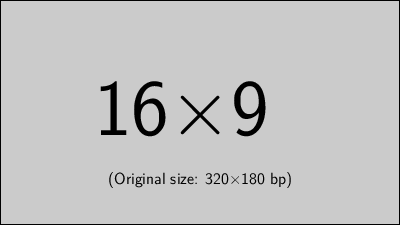
\includegraphics[width=\linewidth]{example-image-16x9}
\caption{This is an example figure with caption. Use the fullwidth environment to make it span the entire width of the page. Lorem ipsum dolor sit amet, consectetur adipiscing elit.}
\label{fig:example}
\end{fullwidth}
\end{figure}


\section{Introduction}

The introduction should supply sufficient background information to allow the reader to understand and evaluate the results of the present study without referring to previous publications on the topic. The introduction should also provide the hypothesis that was addressed or the rationale for the present study. Choose references carefully to provide the most salient background rather than an exhaustive review of the topic.

\textbf{Sectioning commands.}
Use \verb|\section| to get a first-level heading. You can use \verb|\subsection| or just \verb|\textbf| to get a sub-heading. Further sectioning levels, such as \verb|\subsubsection|, etc., are ignored.

Sections \textbf{must} be ordered as follows:

\begin{itemize}
\item Abstract
\item Importance
\item Keywords
\item Introduction
\item Results
\item Discussion
\item Materials and Methods
\item Supplemental Material file list (where applicable)
\item Acknowledgments
\item References
\end{itemize}

\textbf{Citations and References.}
This template uses BibTeX and natbib, so \verb|\citep| and \verb|\citet| such as \citep{caserta:etal:2012}, \citet{johnson:robinson:2016} can be used as usual to produce the correct citation style, and the reference list is generated automatically. In the reference list, references are numbered in the order in which they are cited in the article (citation-sequence reference system). In the text, references are cited parenthetically by number in sequential order. Data that are not published or not peer reviewed are simply cited parenthetically in the text. The \href{https://journals.asm.org/journal/msystems/article-types}{mSystems Instructions to Authors} contain additional guidelines for the reference list and examples of how various types of references should be presented in the manuscript.

\begin{enumerate}[label=(\roman*)]
\item \textbf{References listed in the References section.} The mSystems Instructions to Authors contain examples of the types of items that should be cited in the reference list. Those examples have been reproduced in the template bib file, as have other sample references.

\item \textbf{References cited in the text.} As indicated in the mSystems Instructions to Authors, certain reference types should be cited parenthetically rather than in the reference list. This paragraph shows examples of reference citations as they might appear within the manuscript text instead of in the reference list. A citation of unpublished data should appear as shown here (R.~B. ~Layton and C.~C.~Weathers, unpublished data). A citation of a manuscript submitted for publication should appear as shown here (J.~L.~McInerney, A.~F.~Holden, and P.~N.~Brighton, submitted for publication). Citations of nonpublished abstracts and posters, etc., should appear as shown here (M.~G.~Gordon and F.~L.~Rattner, presented at the Fourth Symposium on Food Microbiology, Overton, IL, 13 to 15 June 1989). For non-U.S.~patent applications, give the date of publication of the application, as shown here (V.~R.~Smoll, 20 June 1999, Australian Patent Office). A website should be cited as shown here for the World Health Organization (\url{https://www.who.int/news-room/detail/17-01-2020-lack-of-new-antibiotics-threatens-global-efforts-to-contain-drug-resistant-infections}). URLs for companies that produce any of the products mentioned in your study or for products being sold may not be included in the article. However, company URLs that permit access to scientific data related to the study or to shareware used in the study are permitted.


\item \textbf{Citations in abstracts.} Since the abstract must be able to stand apart from the article, references cited in it should be clear without recourse to the References section. Use an abbreviated form of citation, omitting the article title, as follows.

\begin{itemize}
\item (P.~S.~Satheshkumar, A.~S.~Weisberg, and B.~Moss, J Virol 87:10700--10709, 2013, doi:10.1128/JVI.01258-13)
\item (J.~H.~Coggin, Jr., p.~93–114, in D.~O.~Fleming and D.~L.~Hunt, ed., \emph{Biological Safety. Principles and Practices,} 4th ed., 2006)
\end{itemize}

\begin{quote}
``\ldots  in a recent report by D. A. Hopwood (mBio 4:e00612-13, 2013, doi:10.1128/mBio.00612-13) \ldots''
\end{quote}

\item \textbf{References related to supplemental material.} If references must be cited in the supplemental material, list them in a separate References section within the supplemental material and cite them by those numbers; do not simply include citations of numbers from the reference list of the associated article. If the same reference(s) is to be cited in both the article itself and the supplemental material, then that reference would be listed in both References sections.

\item \textbf{Citations of data sets and/or code.} To encourage data sharing and reuse, ASM recommends reporting data sets and/or code both in a dedicated “Data availability” paragraph and in the reference list. Examples related to data citation have been reproduced in the template bib file, as have other sample references.
\end{enumerate}

\textbf{Author Warranty.} If accepted for publication, the Work will be made freely available to the public on ASM's \textit{\href{https://journals.asm.org/journal/msystems}{mSystems}} website. ASM will grant the public the nonexclusive right to copy, distribute, adapt, and transmit the published Work for commercial or non-commercial use with proper attribution under the Creative Commons, Attribution license, Version 4.0 (CC-BY). For details, see \url{https://creativecommons.org/licenses/by/4.0/} and \url{https://creativecommons.org/licenses/by/4.0/legalcode}, as well as \url{https://journals.asm.org/author-warranty-and-provisional-license-publish}.

\textbf{\LaTeX{} files.} Authors who prefer to use \LaTeX{} for manuscript preparation may use this Overleaf template. Files from an Overleaf project may be transferred directly from Overleaf to mSystems once for initial manuscript submission. Although a compiled PDF alone is acceptable for initial submission of a manuscript prepared in \LaTeX{}, mSystems requires all \LaTeX{} files from a project to be uploaded at the revision stage. On the mSystems submission site, the .tex file should be classified as a Manuscript Text File. Other supporting files that appear in the Overleaf package (i.e., .bib, .bst, .cls, .ldf, and .sty files) should all be included and classified as `LaTeX Support Files'. Figure files should be classified as Figure files; the usual formatting restrictions apply (see mSystems Instructions to Authors). When the mSystems manuscript record already exists, files must be replaced on the mSystems submission site (\url{https://msystems.msubmit.net}) if modification is required. Contact journal staff with questions related to file conversion in the mSystems manuscript record.

\section{Results}

In the Results section, include the rationale or design of the experiments as well as the results; reserve extensive interpretation  of  the  results  for  the  Discussion  section.  Present the results as concisely as possible in one or more of the following: text, table(s), or figure(s). Data in tables (e.g., cpm of radioactivity) should not contain more significant figures than the precision of the measurement allows. Illustrations (particularly photomicrographs and electron micrographs) should be limited to those that are absolutely necessary to show the experimental findings. Number figures and tables in the order in which they are cited in the text, and be sure to cite all figures and tables. \autoref{fig:example} is just for show, but this sentence shows how a figure could be cited in the text of the manuscript.

The tabularx, booktabs and siunitx packages are loaded by asm-article.cls; see \autoref{tab:example} for an example table. Use \verb|\begin{fullwidth}...\end{fullwidth}| in your table for the table to span the entire width of the page. Shading in the field of tables is allowed, to demonstrate relationships among data. You can use the \verb|\columncolor|, \verb|\rowcolor| or \verb|\cellcolor| commands to do this: allowed color values are \verb|black!20| and \verb|black!30|.

\begin{table}[tp!]
\begin{fullwidth}
\caption{\label{tab:example}Automobile land speed records (GR 5-10)\tnote{a}}
% Use "S" column identifier (from siunitx) to align on decimal point.
% Use "L", "R" or "C" column identifier for auto-wrapping columns with tabularx.
\begin{tabularx}{\linewidth}{S l l >{\columncolor{black!20}}l r L}
\toprule
\headrowfillerT % to fill in the white gap
\headrow \textbf{Speed (mph)} & \textbf{Driver} & \textbf{Car} & \textbf{Engine} & \textbf{Date} & \textbf{Extra comments}\\
\headrowfillerB % to fill in the white gap
\midrule
407.447     & Craig Breedlove & Spirit of America          & GE J47    & 8/5/63  & (Just to demo a full-width table with auto-wrapping long lines) \\
413.199     & Tom Green       & Wingfoot Express           & \cellcolor{black!30}WE J46    & 10/2/64  \\
434.22      & Art Arfons      & Green Monster              & GE J79    & 10/5/64  \\
468.719     & Craig Breedlove & Spirit of America          & GE J79    & 10/13/64 \\
526.277     & Craig Breedlove & Spirit of America          & GE J79    & 10/15/65 \\
536.712     & Art Arfons      & Green Monster              & GE J79    & 10/27/65 \\
555.127     & Craig Breedlove & Spirit of America, Sonic 1 & GE J79    & 11/2/65  \\
576.553     & Art Arfons      & Green Monster              & GE J79    & 11/7/65  \\
600.601     & Craig Breedlove & Spirit of America, Sonic 1 & GE J79    & 11/15/65 \\
622.407     & Gary Gabelich   & Blue Flame                 & Rocket    & \cellcolor{black!20}10/23/70 \\
633.468     & Richard Noble   & Thrust 2                   & \cellcolor{black!30}RR RG 146 & \cellcolor{black!20}10/4/83  \\
763.035     & Andy Green      & Thrust SSC                 & \cellcolor{black!30}RR Spey   & \cellcolor{black!20}10/15/97\\
\bottomrule
\end{tabularx}

\begin{tablenotes}
\item[a] Source is from this website: \url{https://www.sedl.org/afterschool/toolkits/science/pdf/ast_sci_data_tables_sample.pdf}
\end{tablenotes}
\end{fullwidth}
\end{table}

\textbf{File types and formats.}
Illustrations may be continuous-tone images, line drawings, or composites. On initial submission, illustrations may be supplied as PDF files, with the legend on the same page, to assist review. At the modification stage, production quality digital files must be provided, along with text files for the legends. The legends are copyedited and typeset for final publication, not included as part of the figure itself.

All graphics submitted with modified manuscripts should be grayscale or in the RGB color mode. Minimum resolution is 300 dpi for all file types. All images imported into a figure file must be at the correct resolution before they are placed in the file. (For instance, placing a 72-dpi image in a 300-dpi EPS file will not result in the placed image meeting the minimum requirements for file resolution.) Note that publication quality will not be improved by using a resolution higher than the minimum.

All graphics should be submitted at their intended publication size; that is, the image uploaded should be 100\% of its print dimensions so that no reduction or enlargement is necessary. Resolution must be at the required level at the submitted size. Include only the significant portion of an illustration. White space must be cropped from the image, and excess space between panel labels and the image must be eliminated.

\begin{itemize}
\item Maximum figure width: 6.875 inches (ca.~17.4 cm)
\item Maximum figure height: 9.0625 inches (23.0 cm)
\end{itemize}


\section{Discussion}
The Discussion section should provide an interpretation of the results in relation to previously published work and to the experimental system at hand and should not contain extensive repetition of the Results section or reiteration of the introduction. In short papers, the Results and Discussion sections may be combined.

\begin{equation}
\frac{\partial^2 \Phi}{\partial x^2} + \frac{\partial^2 \Phi}{\partial y^2} +
            \frac{\partial^2 \Phi}{\partial z^2} =
            \frac{1}{c^2}\frac{\partial^2\Phi}{\partial t^2}
\end{equation}

Please note that display equations in the Overleaf template may be rendered with a slightly different presentation in the final published (\textit{mSystems}) article.

Lorem ipsum dolor sit amet, consectetur adipiscing elit, sed do eiusmod tempor incididunt ut labore et dolore magna aliqua. Ut enim ad minim veniam, quis nostrud exercitation ullamco laboris nisi ut aliquip ex ea commodo consequat. Duis aute irure dolor in reprehenderit in voluptate velit esse cillum dolore eu fugiat nulla pariatur. Excepteur sint occaecat cupidatat non proident, sunt in culpa qui officia deserunt mollit anim id est laborum.

\begin{equation}
\int_0^\infty e^{-\alpha x^2} \mathrm{d}x =
            \frac12\sqrt{\int_{-\infty}^\infty e^{-\alpha x^2}}
            \mathrm{d}x\int_{-\infty}^\infty e^{-\alpha y^2}\mathrm{d}y =
            \frac12\sqrt{\frac{\pi}{\alpha}}
\end{equation}

Lorem ipsum dolor sit amet, consectetur adipiscing elit, sed do eiusmod tempor incididunt ut labore et dolore magna aliqua. Ut enim ad minim veniam, quis nostrud exercitation ullamco laboris nisi ut aliquip ex ea commodo consequat.

%TC:ignore
\section{Materials and Methods}
The Materials and Methods section should include sufficient technical information to allow the experiments to be repeated. When centrifugation conditions are critical, give enough information to enable another investigator to repeat the  procedure: make of centrifuge, model of rotor, temperature, time at maximum  speed, and centrifugal force ($\times g$ rather than revolutions per minute). For commonly used materials and methods (e.g., media and protein concentration determinations), a simple reference is sufficient. If several alternative methods are commonly used, it is helpful to identify the method briefly as well as to  cite the reference. For example, it is preferable to state ``cells were broken by ultrasonic treatment as previously described (9)'' rather than to state ``cells were broken as previously described (9).'' This allows the reader to assess the method without constant reference  to  previous  publications. Describe  new  methods completely and give sources of unusual chemicals, equipment, or microbial strains. When large numbers of microbial strains or mutants are used in a study, include tables identifying the immediate sources (i.e., sources from whom the strains were obtained)  and  properties  of  the  strains,  mutants,  bacteriophages, and plasmids, etc.

A method or strain, etc., used in only one of several experiments reported in the paper may be described in the Results section or very briefly (one or two sentences) in a table footnote or figure legend. It is expected that the sources from whom the strains were obtained will be identified.

\textbf{Availability of data and materials.} By publishing in mSystems, the authors agree that, subject to requirements or limitations imposed by local and/or U.S. Government laws and regulations, any materials and data that are reasonably requested by others are available from a publicly accessible collection or will be made available in a timely fashion, at reasonable cost, and in limited quantities to members of the scientific community for noncommercial purposes. Similarly, the authors agree to make available computer programs and/or code, originating in the authors’ laboratory, that is the only means of confirming the conclusions reported in the article but that is not available commercially. The program(s) and suitable documentation regarding its (their) use may be provided by any of the following means: (i) as a program transmitted via the Internet, (ii) as an Internet server-based tool, or (iii) as a compiled or assembled form on a suitable medium. The authors guarantee that they have the authority to comply with this policy either directly or by means of material transfer agreements through the owner. ASM asks authors to assert this in a “Data availability” paragraph, which should appear at the end of the Materials and Methods section (or at the end of the text) of their submitted manuscript.

Therefore, a condition of publication in mSystems is that authors make data fully available and without restriction, except in rare circumstances. Data availability will be confirmed prior to publication and must be provided during the modification stage, if not before. Furthermore, data must be made available, upon request, for peer review. See \href{https://journals.asm.org/open-data-policy}{Data Policy}.

\textbf{Data citation.}
To promote reproducibility, ASM expects researchers to identify and cite data sets and/or code used in their experiments and studies. These may be large or complex data sets that can include, but are not limited to, data from microarray, genomic, structural, proteomic, or video imaging analyses. \textbf{Authors should cite both the data set repository and the published article in which the data set and/or code was originally described.} Citations of data should be included in the reference list with persistent unique identifiers (e.g., active DOIs, accession numbers, etc.). If computer code or software was created to generate results or interpret data, then a statement to that effect should be included in the ``Data availability'' paragraph. For cases in which the software is publicly available (e.g., \href{http://tree.bio.ed.ac.uk/software/figtree/}{FigTree} to generate phylogenetic trees), the URL of the software informational page should be provided. \textbf{It is preferred that authors use established, publicly available \href{https://journals.asm.org/list-data-repositories}{data type-specific repositories}.} If there is no appropriate repository available, general publicly available repositories should be used (e.g., \href{https://datadryad.org/stash}{Dryad}, \href{https://figshare.com/}{figshare}, etc.).

\section{Supplemental Material}
Guidelines for supplemental material appear in the Instructions to Authors. This section of the paper should include legends for any supplemental material that is intended for posting. Such supplemental material must be submitted with the manuscript. Files can be added to the submission at the publisher's submission site. Here is a list of sample legends for supplemental material:

\textbf{FIG S1.} Supplemental file 1 is a figure that shows results related to the study, although the study stands on its own. This legend for the figure may include multiple sentences.

\textbf{FIG S2.} Supplemental file 2 is a figure that shows results related to the study, although the study stands on its own. This legend for the figure may include multiple sentences.

\textbf{FIG S3.} Supplemental file 3 is a figure that shows results related to the study, although the study stands on its own. This legend for the figure may include multiple sentences.

\textbf{TABLE S1.} Supplemental file 4 is a large table that shows results related to the study, although the study stands on its own. This legend for the table may include multiple sentences.

\textbf{TABLE S2.} Supplemental file 5 is a complex table that shows results related to the study, although the study stands on its own. This legend for the supplemental material may include multiple sentences.


\section{Acknowledgments}
Statements regarding sources of direct financial support (e.g., grants, fellowships, and scholarships, etc.) should appear in the Acknowledgments. A funding statement indicating what role, if any, the funding agency had in your study (for example, ``The funders had no role in study design, data collection and interpretation, or the decision to submit the work for publication.'') may be included. Funding agencies may have specific wording requirements, and compliance with such requirements is the responsibility of the author. In cases in which research is not funded by any specific project grant, funders need not be listed, and the following statement may be used: ``This research received no specific grant from any funding agency in the public, commercial, or not-for-profit sectors.'' Statements regarding indirect financial support (e.g., commercial affiliations, consultancies, stock or equity interests, and patent-licensing arrangements) are also allowed. It is the responsibility of authors to provide a general statement disclosing financial or other relationships that are relevant to the study.  Recognition of personal assistance should be given as a separate paragraph, as should any statements disclaiming endorsement or approval of the views reflected in the paper or of a product mentioned therein. In addition to acknowledging sources of financial support in the manuscript, authors should list any sources of funding in response to the Funding Sources question on the online submission form, providing relevant grant numbers where possible, and the authors associated with the specific funding sources. In the event that your submission is accepted, the funding source information provided in the submission form may be published, so please ensure that all information is entered accurately and completely. (It will be assumed that the absence of any information in the Funding Sources fields is a statement by the authors that no support was received.)

Authors may include a statement that specifies contributor roles as a separate paragraph in the Acknowledgments section. ASM encourages transparency in authorship by publishing author contribution statements using the CRediT taxonomy as recommended by \href{https://casrai.org/credit/}{CASRAI}. For some manuscript types, authors have the option of assigning CRediT roles during the online submission process.

\textbf{Please read the \href{https://journals.asm.org/journal/msystems/submission-review-process}{Instructions to Authors} or browse the \href{https://journals.asm.org/journal/msystems/faq}{FAQs} for further details.}

\nocite{*}
\bibliography{asm-sample}
%TC:endignore

\end{document}
